\chapter{Additional Simulation Results}
\label{sec:additional_simulation_results}
Figures~\ref{fig:simulation_bias_combined_a_p4}--\ref{fig:simulation_coverage_combined_a_p4} 
report the results of the simulation study for the four-covariate case. 
The additional results for the four-covariate case lead to the same overall conclusions as in 
the two-covariate setting. Figure~\ref{fig:simulation_bias_combined_a_p4} reports the bias, 
Figure~\ref{fig:simulation_standard_error_combined_a_p4} reports the standard error, and 
Figure~\ref{fig:simulation_coverage_combined_a_p4} reports the coverage. 
Within each figure, the first two rows correspond to the weak unmeasured confounding setting 
($c_U=1$), and the last two rows correspond to the strong unmeasured confounding setting 
($c_U=2$). The first and third rows correspond to $\tau_F=1$, while the second and fourth 
rows correspond to $\tau_C=0.3$. The columns correspond to the $N$ to $T$ ratio, with 
panels (A), (D), (G), and (J) showing $\rho=5$, panels (B), (E), (H), and (K) showing 
$\rho=10$, and panels (C), (F), (I), and (L) showing $\rho=50$. 
In particular, both \texttt{FE-MSM} and \texttt{SeqGPLVM-MSM} 
still improve over the naive \texttt{IPTW} estimator, while \texttt{FE-MSM} remains uniformly 
closer to \texttt{IPTW-True} and exhibits smaller estimated standard errors than \texttt{SeqGPLVM-MSM}. 
However, increasing the number of observed covariates from \(d_X=2\) to \(d_X=4\) does not lead to a systematic 
finite-sample improvement. Across scenarios, the \(d_X=4\) results are generally associated with larger average 
standard errors (Figure~\ref{fig:simulation_standard_error_combined_a_p4}). 
Although coverage occasionally improves in the more difficult settings, especially under stronger unmeasured 
confounding, these improvements appear to be driven mainly by wider intervals rather than smaller bias 
(Figures~\ref{fig:simulation_bias_combined_a_p4} and~\ref{fig:simulation_coverage_combined_a_p4}, panels (G)--(L)). 
As in the main results, the most challenging regime remains the short-panel setting with \(\rho=50\), 
particularly for smaller sample sizes, where the performance of both adjusted estimators deteriorates especially 
for \texttt{SeqGPLVM-MSM} (Figures~\ref{fig:simulation_bias_combined_a_p4}--\ref{fig:simulation_coverage_combined_a_p4}, panels (C), (F), (I), and (L)).
\begin{figure}[!tbp]
    \centering
    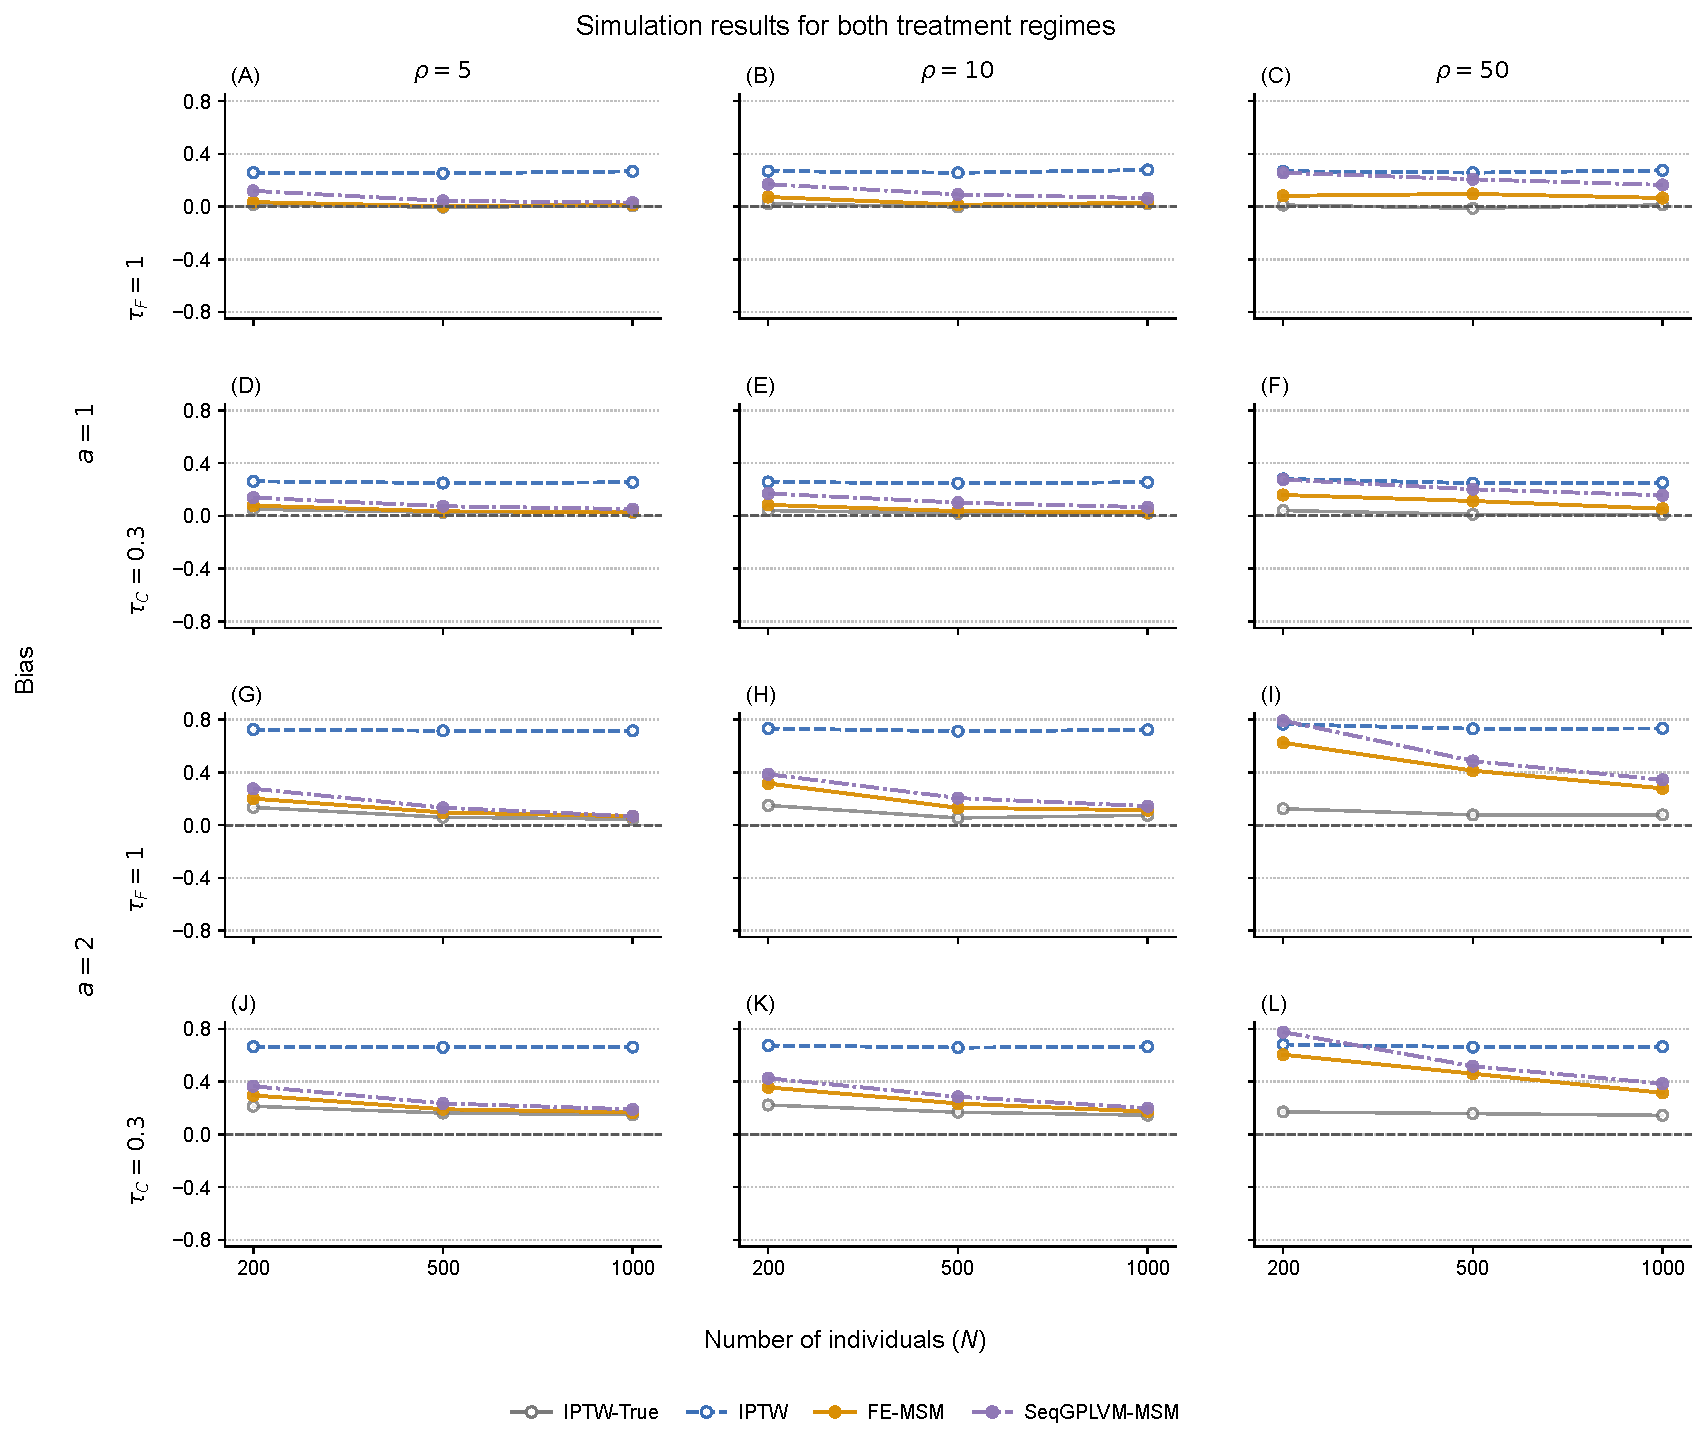
\includegraphics[width=\textwidth]{figures/build/simulation_bias_combined_a_p4.pdf}
    \caption{Simulation bias for the four-covariate case. The panels report bias for $c_U=1$ and $c_U=2$, for $\tau_F=1$ and $\tau_C=0.3$, across sample sizes $N$ and ratios $\rho = N/T$.}
    \label{fig:simulation_bias_combined_a_p4}
\end{figure}

\begin{figure}[!tbp]
    \centering
    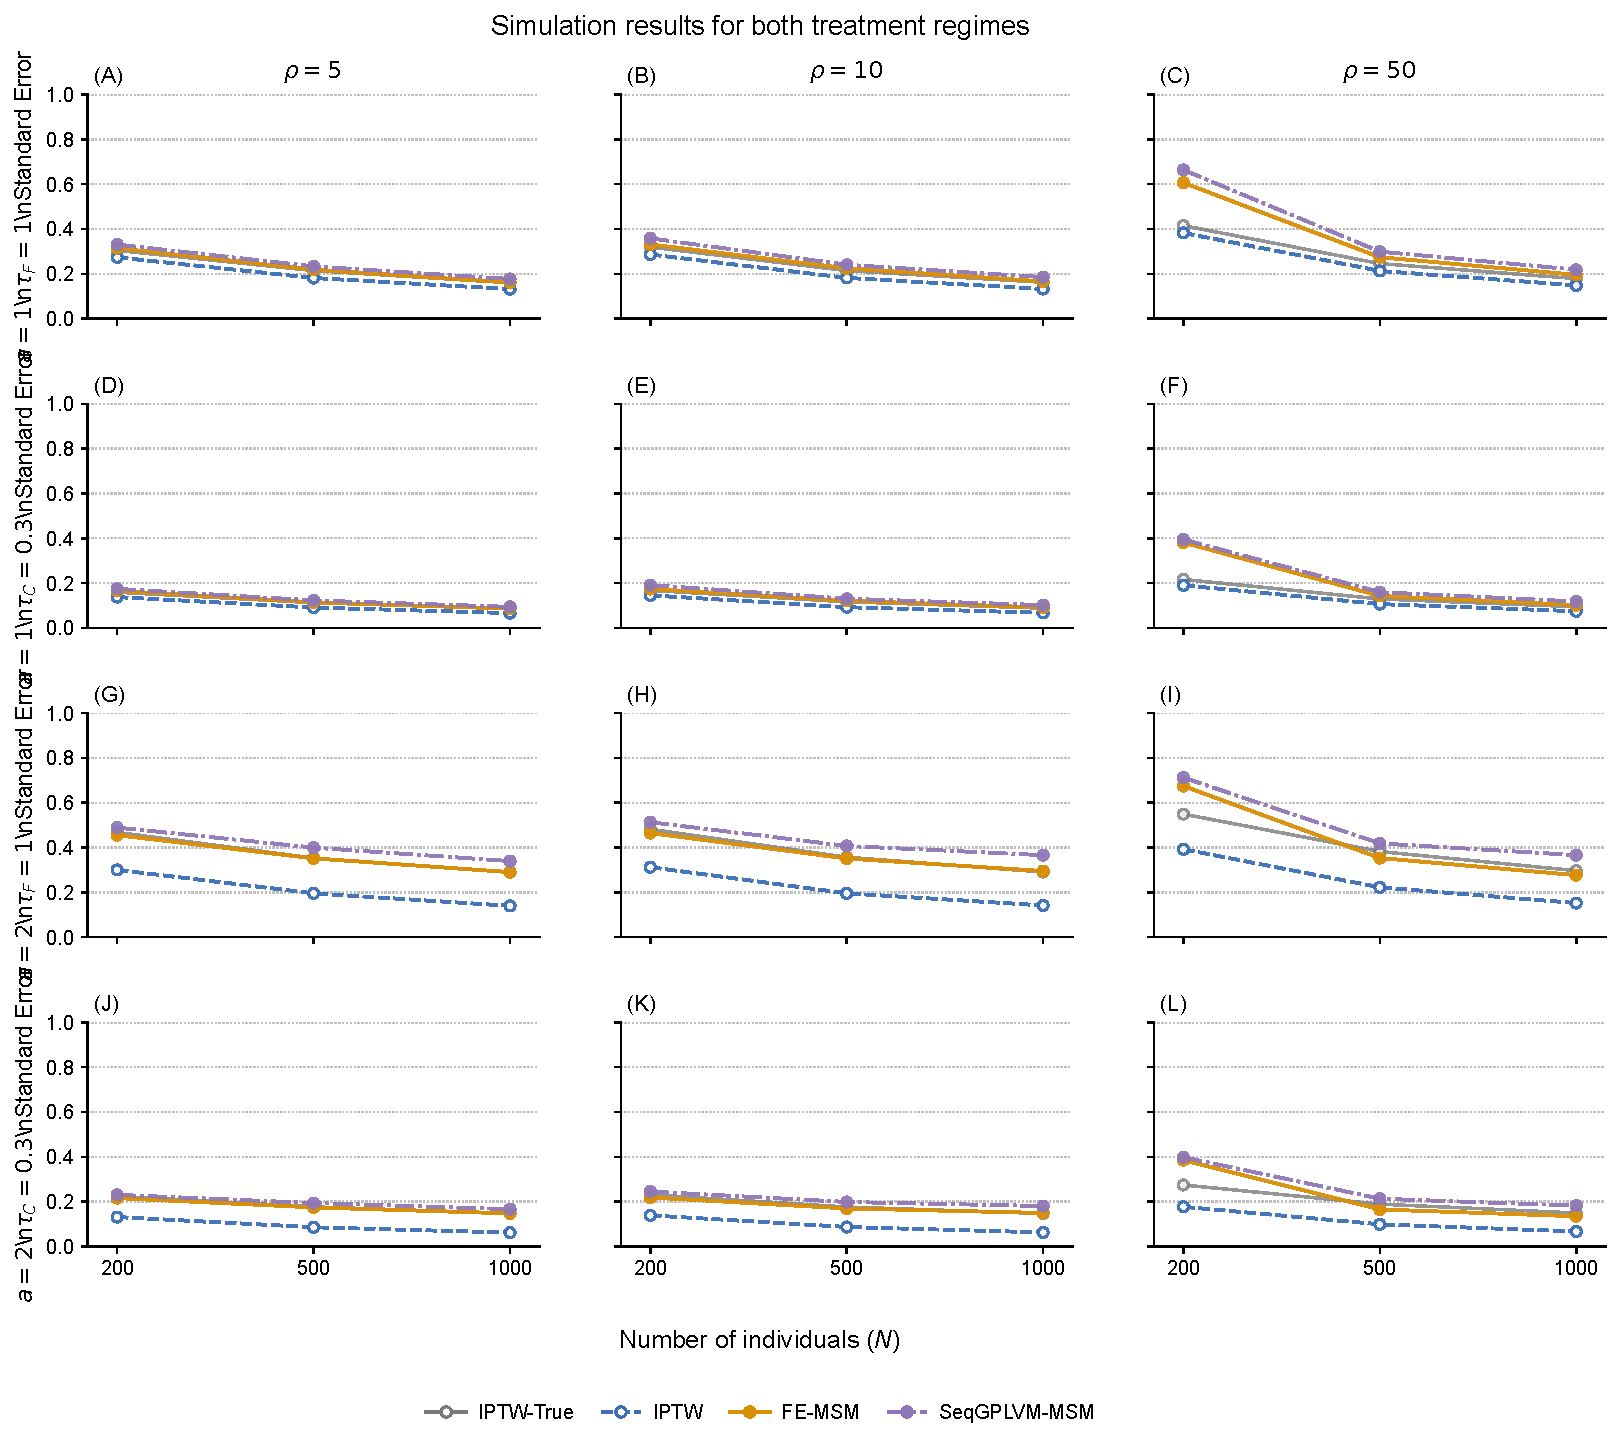
\includegraphics[width=\textwidth]{figures/build/simulation_standard_error_combined_a_p4.pdf}
    \caption{Simulation standard error for the four-covariate case. The panels report standard error for $c_U=1$ and $c_U=2$, for $\tau_F=1$ and $\tau_C=0.3$, across sample sizes $N$ and ratios $\rho = N/T$.}
    \label{fig:simulation_standard_error_combined_a_p4}
\end{figure}

\begin{figure}[!tbp]
    \centering
    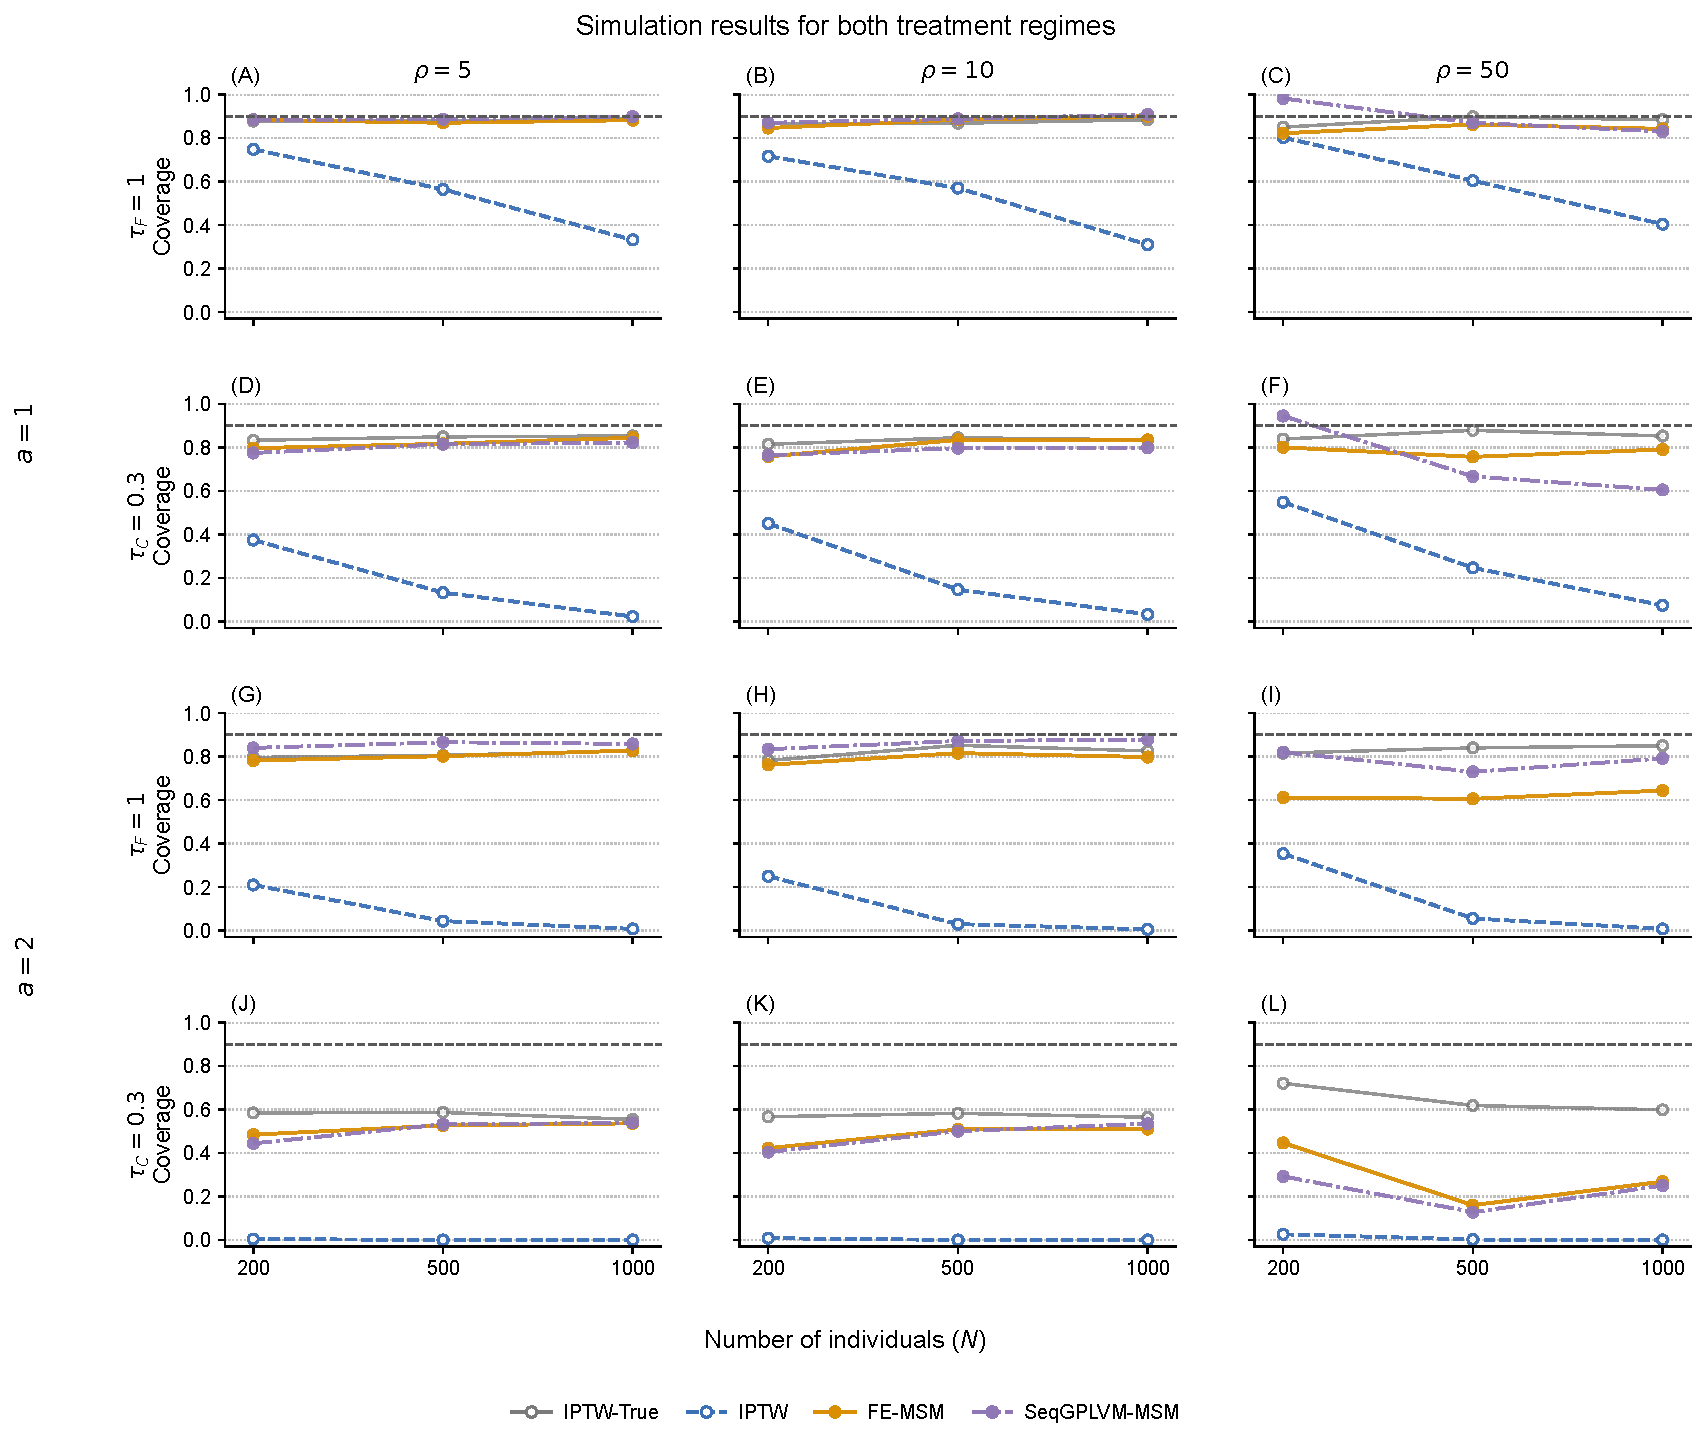
\includegraphics[width=\textwidth]{figures/build/simulation_coverage_combined_a_p4.pdf}
    \caption{Simulation coverage for the four-covariate case. The panels report coverage of the 90\% confidence intervals for $c_U=1$ and $c_U=2$, for $\tau_F=1$ and $\tau_C=0.3$, across sample sizes $N$ and ratios $\rho = N/T$.}
    \label{fig:simulation_coverage_combined_a_p4}
\end{figure}
